\chapter{Convolutional Neural Network} \label{chap:cnn}
\acrfull{cnn} is a type of \acrlong{nn} that is specialized in analyzing visual imagery and natural language processing. \acrshort{cnn}s are feedforward, sparsely connected \acrshort{nn} structured as a pipeline of layers \cite{abdelouahab_accelerating_2018}. It has shown explemplary performance on serveral competitions related to Computer Vision and Image Processing \cite{khan_survey_2020}. We explore in this chapter the different aspects of a \acrshort{cnn} and what optimizations can be made to reduce its size and its computational complexity.

Section \ref{sec:layer} introduces the building blocks of a \acrshort{cnn}. We start from the first and most simple element, the perceptron. From this first step, we explore how to use it to make more complex layers that can perform more complex functions. We also detail the other layers required to improve the efficiency of the model, such as pooling.

The second section is concentrated on the training of a \acrshort{cnn}. We explain briefly the backpropagation algorithm, which consists of a forward propagation (section \ref{subs:trainforward}) and a back propagation (section \ref{subs:trainbackward}).

The third section details how we can use the layer from section \ref{sec:layer} to build efficient network. We discuss about state-of-art networks like AlexNet, VGG16, ResNet and MobileNetV2.

The fourth section details the optimization we can make on the convolution operation to have a faster inference on \acrshort{fpga}. We focus on the algorithmic and model optimizations.
%
%
\section{Layers} \label{sec:layer}
A layer is a high-level building block in a \acrshort{dl} network. It is a set of operations, weights, and non-linear functions. The result of the layer can be either used as input for the following layer or either as the final output of the network. We can, therefore, define a \acrshort{cnn} as a pipeline of layers, and a network is built by stacking layers. We begin our understanding of the layer theory in section \ref{subs:perceptron} by explaining the perceptron, the simplest element of a neural network.
%
%
\subsection{Perceptron} \label{subs:perceptron}
The perceptron was developed in 1957 by \textcite{rosenblatt_perceptron_1958}. The idea is to compare the computational model to a human brain which is composed of a large number of units called neurons. A neuron receives an information and when its threshold is reached (we say the neuron fires), this information is released and transmitted to other neurons \cite{rosenblatt_perceptron_1958, matteucci_artificial_2019}.

\begin{figure}
    \centering
    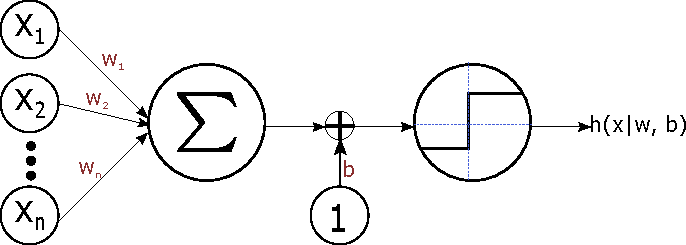
\includegraphics[width=0.8\textwidth]{perceptron.pdf}
    \caption{The Perceptron}
    \label{fig:perceptron}
\end{figure}
%
This neuron in a human brain corresponds to a perceptron in the computational model. It is composed of $n_{in}$ inputs $\boldsymbol{x} = \{ x_1, ... x_{n_{in}} \}$, $n_{in}$ weights $\boldsymbol{w}$ and a bias $b$. Figure \ref{fig:perceptron} illustrates the working principle of a perceptron. When a perceptron received an input vector $\boldsymbol{x}$, a weighted sum of this vector is performed. If its result is higher than the threshold (controlled by $b$), the perceptron is \textquote{activated} and its output becomes a non-zero value.
Equation \ref{eq:perceptron} represents the mathematical formula of the perceptron where $h$ is the activation function of the formula developed in Equation \ref{eq:step} \cite{matteucci_artificial_2019}.
%
\begin{equation}
    h ( \boldsymbol{x} | \boldsymbol{w}, b) = h \left( \sum^{n_{in}}_{i=1} x_i \cdot w_i + b \right) = h \left( \boldsymbol{w}^{T} \cdot \boldsymbol{x} + b \right)
    \label{eq:perceptron}
\end{equation}
%
\begin{equation}
    h ( \boldsymbol{w}^{T} \cdot \boldsymbol{x} + b) = \begin{cases} 1, & \mbox{if } \boldsymbol{w}^{T} \cdot \boldsymbol{x} + b > 0 \\ 0, & \mbox{Otherwise} \end{cases}
    \label{eq:step}
\end{equation}

As the perceptron performs a weighted sum, those weights can be learned to perform a task of interest. However, this model is limited by the functions it can achieve. In Section \ref{subs:fcl}, we discover how we can use multiple perceptrons to create a \textbf{fully-connected layer} to learn more complex functions.

%
\subsection{Activation of a perceptron} \label{subs:acti}
In order to decide if a perceptron is activated or not (if its threshold is reached), an activation function needs to be defined. However, to use this function in a \acrshort{dl} model and be able to apply the back-propagation algorithm (will be further detailed in Section \ref{sec:train}), this function needs to be differentiable \cite{lecun_backpropagation_1989}. Indeed, during the optimization of the network, the gradient of the activation function is computed. Therefore, Equation \ref{eq:step} cannot be used as the activation function because of its zero gradient and the learning does not converge.  Various activation functions have been proposed with different properties, as illustrated in Figure \ref{fig:acti}. According to \textcite{khan_survey_2020}, the choice of an appropriate activation function can accelerate the learning phase and some activations decrease the computational complexity \cite{krizhevsky_imagenet_2012}.
%
\begin{figure}
    \centering
    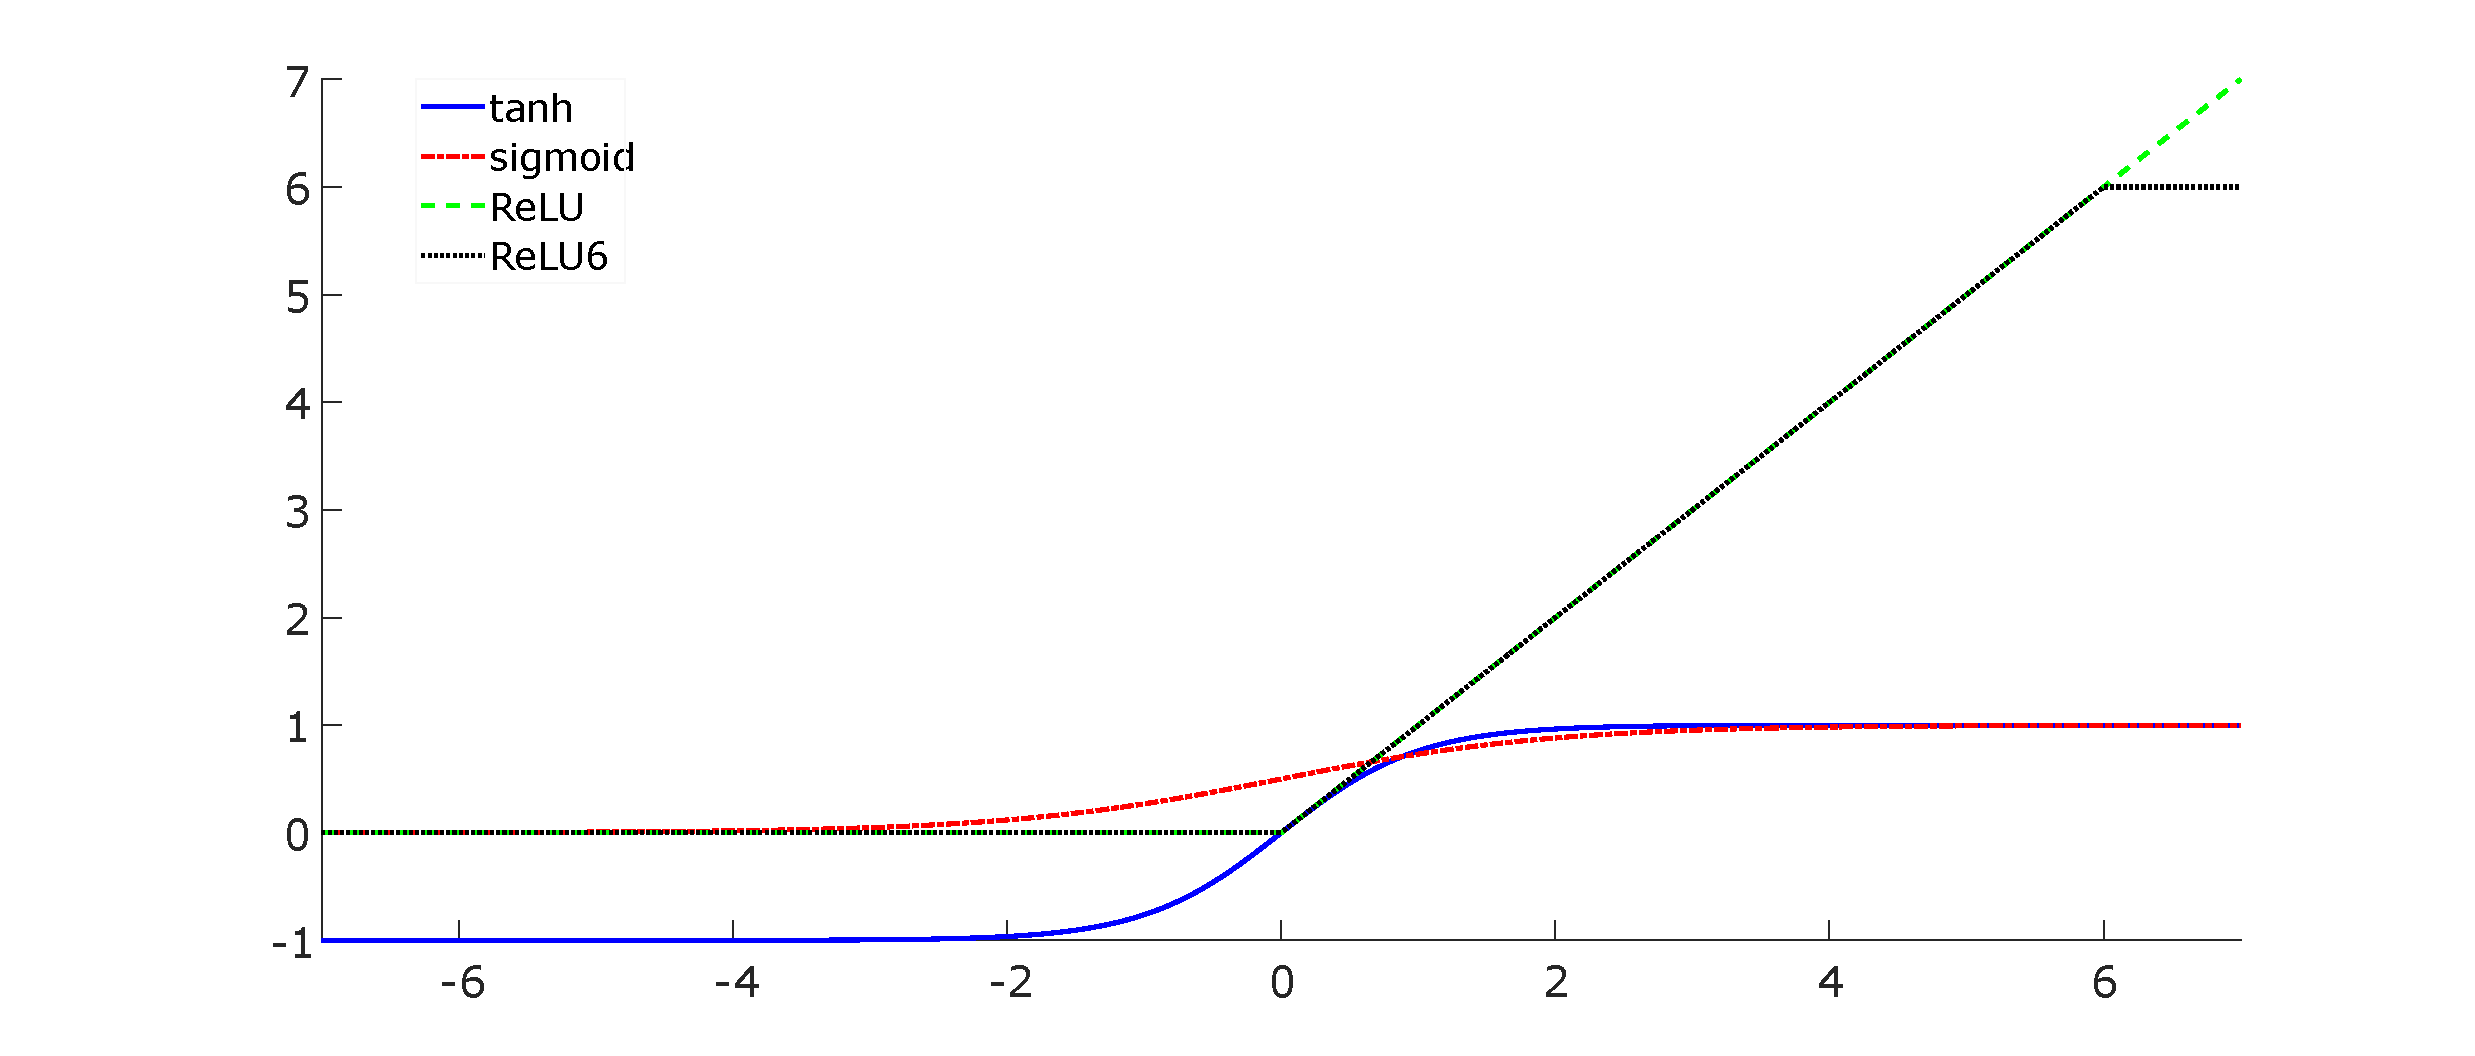
\includegraphics[width=\textwidth]{actifun.pdf}
    \caption{Activation functions}
    \label{fig:acti}
\end{figure}
%
\subsubsection{Sigmoid and Hyperbolic Tangent (Tanh)}
$Sigmoid$ and $Tanh$ are both smooth functions that can be described by equations \eqref{eq:sigmoid} and \eqref{eq:tanh} \cite{krizhevsky_imagenet_2012}.
%
\begin{equation}
    h(x) = \frac{1}{1 + e^{-x}}
    \label{eq:sigmoid}
\end{equation}
%
\begin{equation}
    h(x) = \frac{e^{x} - e^{-x}}{e^{x} + e^{-x}}
    \label{eq:tanh}
\end{equation}
%
These two activation functions can be seen in Figure \ref{fig:acti}. They both limith the $\mathbb{R}$ domain into a narrower domain, $[0, 1]$ for $Sigmoid$, and $[-1, 1]$ for the $Tanh$. However, they also saturate at the asymptotes, which means that often their gradient is close to 0 \cite{glorot_understanding_2010}. As the back-propagation algorithm (see Section \ref{sec:train}) requires gradient multiplication, gradient far away from the output vanishes (close to 0) and deep models do not learn: it is the \textbf{vanishing gradient problem} \cite{goodfellow_deep_2016, khan_survey_2020, maas_rectier_2014}.
%
\subsubsection{ReLU}
In order to overcome this vanishing gradient problem, the Rectified Linear Unit (ReLU) which is defined by Equation \eqref{eq:relu} has been developed by \textcite{krizhevsky_imagenet_2012}.
%
\begin{equation}
    h(x) = max(0, x)
    \label{eq:relu}
\end{equation}
%
This function increases the learning and computational speed compared to the $Tanh$ and $Sigmoid$ functions and improves the propagation gradient efficiency (to avoid vanishing or exploding gradient) \cite{maas_rectier_2014, abdelouahab_accelerating_2018}. However, in this function, some perceptrons can become inactive which means that their output is zero for all input. It is called the \textbf{dying neuron problem} which decreases the model capacity \cite{matteucci_artificial_2019}. A solution would be to discard these inactive neurons by transforming the ReLU into a leaky ReLU \cite{maas_rectier_2014} activation function for example.

We can also use the dying neuron property to learn sparse features earlier. It has been done by \textcite{krizhevsky_convolutional_nodate} by setting an upper bound to the ReLU output. For example, in the work, the output is described by Equation \eqref{eq:relu6} and this activation function is called ReLU6 because the range is limited to $[0, 6]$. ReLU has also the advantage to be designed for fixed-point operations and quantization approaches (which will be more described in Section \ref{subsec:mdopti}), instead of floating-point operations. Indeed, floating-point operations, especially on \acrshort{fpga}, are less efficient in terms of hardware utilization and power consumption \cite{david_hardware_2007}. It means that if for example the output $ \in [0, 6]$, the number of bits for the integer part can be limited to 3 bits. The accuracy of the model can thus be increased by assigning the other available bits to the decimal part. For example, ReLU6 is used in model that aims mobile and embedded platforms like MobileNet \cite{howard_mobilenets_2017}. In this work, the ReLU6 activation function is used.
%
\begin{equation}
    h(x) = max(0, x, 6)
    \label{eq:relu6}
\end{equation}

%
\subsection{Fully Connected layer} \label{subs:fcl}
The perceptron of section \ref{subs:perceptron} can be considered as a linear classifier for which the decision boundary is the hyperplane, as seen in equation \eqref{eq:linearclassifer}.
%
\begin{equation}
    b + w_1 \cdot x_1 + ... + w_{n_{in}} \cdot x_{n_{in}} = 0
    \label{eq:linearclassifer}
\end{equation}
%
We can understand why the perceptron is limited because it has only a linear decision boundary. For example, we can implement the AND and OR Boolean functions using a perceptron, but it is impossible to learn the XOR function. To have a non-linear model, we must use a topology of perceptrons. The topology is composed of layers of perceptrons, where each layer, in the case of a \acrshort{cnn}, is called a \textbf{fully-connected layer}. We can see an example in figure \ref{fig:fcn}.
%
\begin{figure}
    \centering
    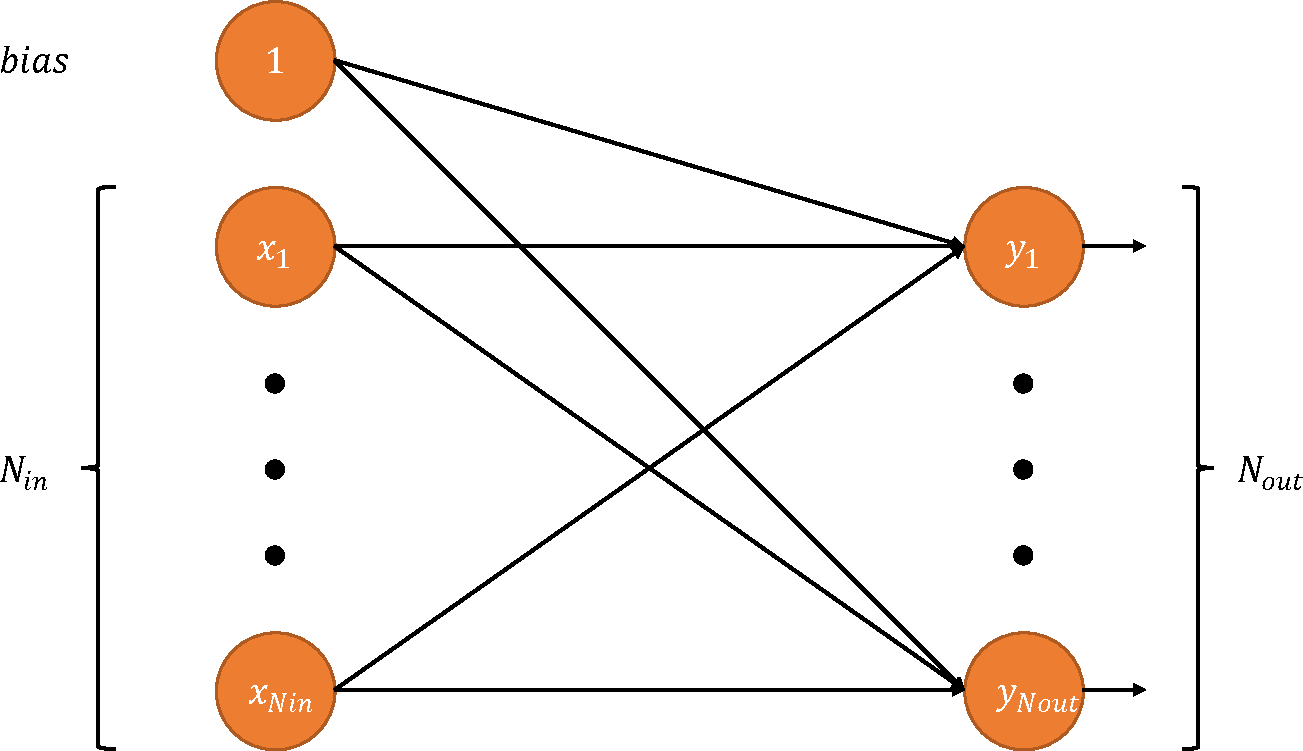
\includegraphics[width=\textwidth]{fcl.pdf}
    \caption{A fully connected layer}
    \label{fig:fcn}
\end{figure}

In the fully-connected layer, each neuron is connected to all the inputs or neurons of previous layers (as the name suggests). Usually, the fully-connected layers are placed at the end of the \acrshort{cnn}. It takes the extracted features from the previous layersas input, which are converted as a one-dimension output \acrshort{fm}. Afterwards, it makes a non-linear classification of them \cite{khan_survey_2020}.

A fully-connected layer is characterized by the number of neurons, activation functions, and the values of weights. The output vector $\boldsymbol{y}$ can be expressed using equation \eqref{eq:fcn}, where $\boldsymbol{x}$ is the vector of the input of the layer and $x_0 = 1$ is the bias;   $\boldsymbol{w}$ is the vector of all the weights of the layer ($w^i_*$ are the weights of the ith perceptron and $w^*_0$ are the biases); $h$ is the activation function of the layer.
%
\begin{equation}
    \boldsymbol{y} = h(\boldsymbol{w}^T \boldsymbol{x}) \Leftrightarrow \forall o \in \{ 1, ..., N_{out} \} : y_o = h(\sum^{N_{in}}_{i=0} w^o_i \cdot x_i)
    \label{eq:fcn}
\end{equation}
%
As we have seen that perceptrons can be used to construct non-linear classifier, we see in the next section \ref{subs:2dconv} the main operation in the \acrshort{cnn}: the \textbf{convolution}, which extracts the feature from input images.

%
\subsection{Convolution layer} \label{subs:2dconv}
In a \acrshort{cnn}, the \textbf{convolutional layer} carries out the feature extraction process of the input image, also called the input \acrfull{fm}. It is the main operation in a \acrshort{cnn} and it is the layer that gives the network its name. The first layer extracts low-level features of the input \acrshort{fm} and the deepest layers use the low-level features to build high-level ones \cite{goodfellow_deep_2016}.

An input image is characterized by 3 parameters: \textbf{$N_{ix}$} the width, \textbf{$N_{iy}$} the height, and \textbf{$N_{if}$} the depth. We can illustrate then the input \acrshort{fm} as a cuboid composed of layers of pixels. An illustration is presented in figure \ref{fig:notation:ifm}.
The convolution layer correlates therefore input \acrshort{fm} and a 4D filter, to produce output \acrshort{fm}, which contains the high-level features \cite{zhao_towards_2018}. The output \acrshort{fm} is also characterized by its width $N_{ox}$, its height $N_{oy}$ and its depth $N_{of}$. We can also see a general output \acrshort{fm} in figure \ref{fig:notation:ofm}. As a result, the filter consists of $N_{of}$ kernels, where each kernel has size $N_{kx} \times N_{ky} \times N_{if}$, that we can see in figure \ref{fig:notation:k}).
%
\begin{figure}
    \centering
    %
    \begin{subfigure}{.32\textwidth}
    \centering
    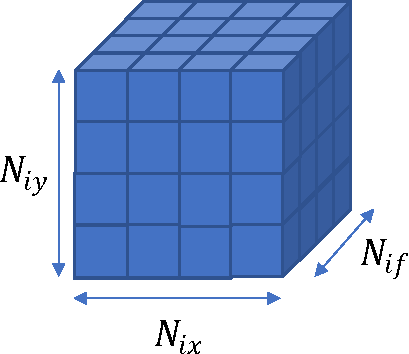
\includegraphics[width=\linewidth]{notifm.pdf}
    \caption{kernel-wise pruning}
    \label{fig:notation:ifm}
    \end{subfigure}
    %
    \begin{subfigure}{.32\textwidth}
    \centering
    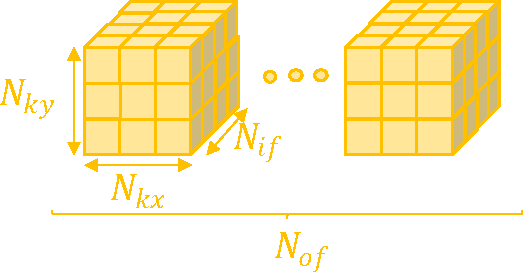
\includegraphics[width=\linewidth]{notk.pdf}
    \caption{Convolution kernel}
    \label{fig:notation:k}
    \end{subfigure}
    %
    \begin{subfigure}{.32\textwidth}
    \centering
    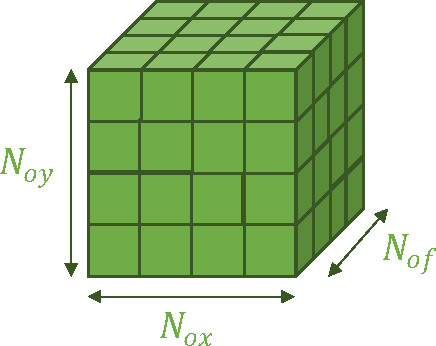
\includegraphics[width=\linewidth]{notofm.pdf}
    \caption{Output \acrshort{fm}s}
    \label{fig:notation:ofm}
    \end{subfigure}
    %
    \caption{Volumes involved in the convolution operations}
    \label{fig:notconv}
\end{figure}

Convolution is a specialized kind of linear operation. The convolution operation happens as follows. Each kernel acts like a sliding window on the input \acrshort{fm}. We extract a chunk of pixels of the same size of the kernel in the input \acrshort{fm} and perform an element-wise multiplication with the chunk of data and the kernel. We sum up the computed pixels to obtain one output pixel. Sliding this kernel on the input \acrshort{fm} will produce a channel of the output \acrshort{fm}, where the output pixel at position $(x, y)$ corresponds to the movement of the sliding window from the top left of the input \acrshort{fm}. Since one kernel produces one channel of the output \acrshort{fm}, having $N_{of}$ kernels produces then $N_{of}$ channels. An illustration of the convolution operation is in figure \ref{fig:convolution}.
%
\begin{figure}
    \centering
    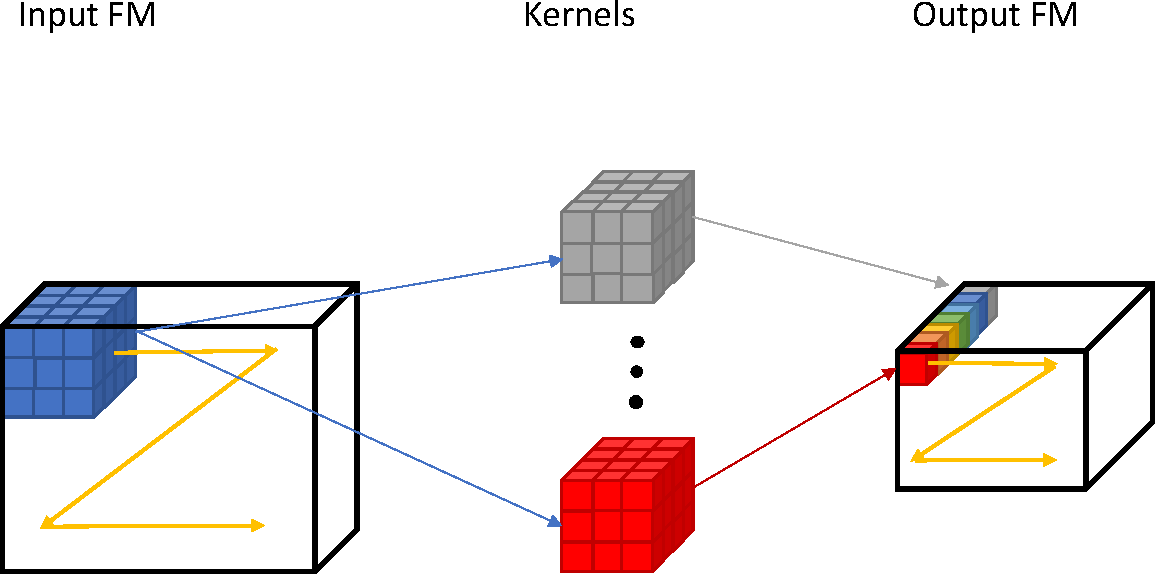
\includegraphics[width=\textwidth]{conv.pdf}
    \caption{Convolution operation}
    \label{fig:convolution}
\end{figure}

Except for $1 \times 1$ kernels, the sliding window can not cover all input pixels, and then there is a spatial reduction between the input and output \acrshort{fm}s, while there is an increase in the number of channel. However, we can keep the same dimensions using \textit{padding} on the boundary. It means that we pad the edges with extra pixels (usually of value 0).

Moreover, each time the sliding window performs a convolution, it shifts in the input \acrshort{fm}. The amount, by which the filter shifts, is called the \textit{stride} and it is initially set to 1. If we increase the stride, we can reduce the spatial dimensions of the output \acrshort{fm}. For example, if we use padding and a stride of 2, $\frac{N_{ix}}{N_{ox}} = \frac{N_{iy}}{N_{oy}} = \frac{1}{2}$, and the output \acrshort{fm} has 4 times fewer pixels. In section \ref{subs:pooling}, we introduce a new layer than can also reduce the spatial dimensions of the output \acrshort{fm}.

Finally, we can express the convolution operations mathematically as in equation \eqref{eq:conv}.
%
\begin{equation}
    \begin{split}
        \forall ox &\in \{ 1, ..., N_{ox} \}, oy \in \{ 1, ..., N_{oy} \}, of \in \{ 1, ..., N_{of} \} : \\
        FM_O[ox, oy, oc] &= \sum^{N_{if}}_{if=1}
        \sum^{N_{kx}}_{kx=1}
        \sum^{N_{ky}}_{ky=1}
        FM_I[ox \cdot S + kx - \lfloor \frac{N_{kx}}{2} \rfloor,  oy \cdot S + ky - \lfloor \frac{N_{ky}}{2} \rfloor, if] \cdot
        W^{of}_{if}[kx, ky]
    \end{split}
    \label{eq:conv}
\end{equation}

If we compare the convolutional layer with the fully-connected layer, the convolutional layer allows a sparse interaction (the kernel is smaller than the input), parameter sharing (we use the same parameter for more than one function) and equivariant representation (for some transformation, a change in the input reflects the same change in the output) \cite{goodfellow_deep_2016}. To illustrate weight sharing, in AlexNet \cite{krizhevsky_imagenet_2012}, 94\% of the weights are used in the fully-connected layers. But as said earlier, convolution is a computationally heavy operation. 90\% of the arithmetic operations are done in the convolutional layer.

As the convolution has a huge arithmetic complexity, we see in the following section \ref{subs:dsc} an alternate way to perform convolution to reduce this.

%
\subsubsection{Depthwise Separable Convolution}  \label{subs:dsc}
\acrfull{dsc} was first introduced by \textcite{sifre_ecole_2014}. According to \textcite{chollet_xception_2017}, \textquote{\textit{A depthwise separable convolution consists in a \textbf{depthwise convolution}, i.e. a spatial convolution performed independently over each channel of an input, followed by a \textbf{pointwise convolution}, i.e. a $1 \times 1$ convolution, projecting the channel's output by the depthwise convolution onto a new channel space}}.

It means that the \acrshort{dsc} is composed of a depthwise convolution followed by a pointwise convolution as illustrated in Figure \ref{fig:dsc}. This alternative form of convolution has been developed to reduce efficiently the arithmetic complexity, in exchange of a limited loss of accuracy \cite{liu_fpga-based_2019}. As a result, the \acrshort{dsc} has significantly fewer parameters and operations with respect to the standard convolution. Equations \eqref{eq:descopred} and \eqref{eq:descwgred} are used to calculate the reduction factors on weigths and on operations respectively, where $F_{*}$ are the factors of reduction, $W_{sc}$ and $O_{sc}$ are the weights and operations required for a standard convolution, and $W_{dsc}$ and $O_{dsc}$ are the weights and operations required for a \acrshort{dsc} \cite{liu_fpga-based_2019}.
%
\begin{equation}
    F_w = \frac{W_{dsc}}{W_{sc}} =
    \frac{N_{kx} \times N_{ky} \times N_{if} + N_{if} \times N_{of}}{N_{kx} \times N_{ky} \times N_{if} \times N_{of}} =
    \frac{1}{N_{of}} + \frac{1}{N_{kx} \times N_{ky}}
    \label{eq:descopred}
\end{equation}
\begin{equation}
    \begin{split}
        F_o &= \frac{O_{dsc}}{O_{sc}} = \frac{N_{kx} \times N_{ky} \times N_{if} \times N_{ox} \times N_{oy} + N_{if} \times N_{of} \times N_{ox} \times N_{oy}}{N_{kx} \times N_{ky} \times N_{if} \times N_{of} \times N_{ox} \times N_{oy}} \\
        &= \frac{1}{N_{of}} + \frac{1}{N_{kx} \times N_{ky}}
    \end{split}
    \label{eq:descwgred}
\end{equation}

Using equation \eqref{eq:descopred} and equation \eqref{eq:descwgred} and $3 \times 3$ kernels, the reduction of computation and parameters in comparison with the standard convolution is about 9 times \cite{zhang_channel_2019}.
%
\begin{figure}
    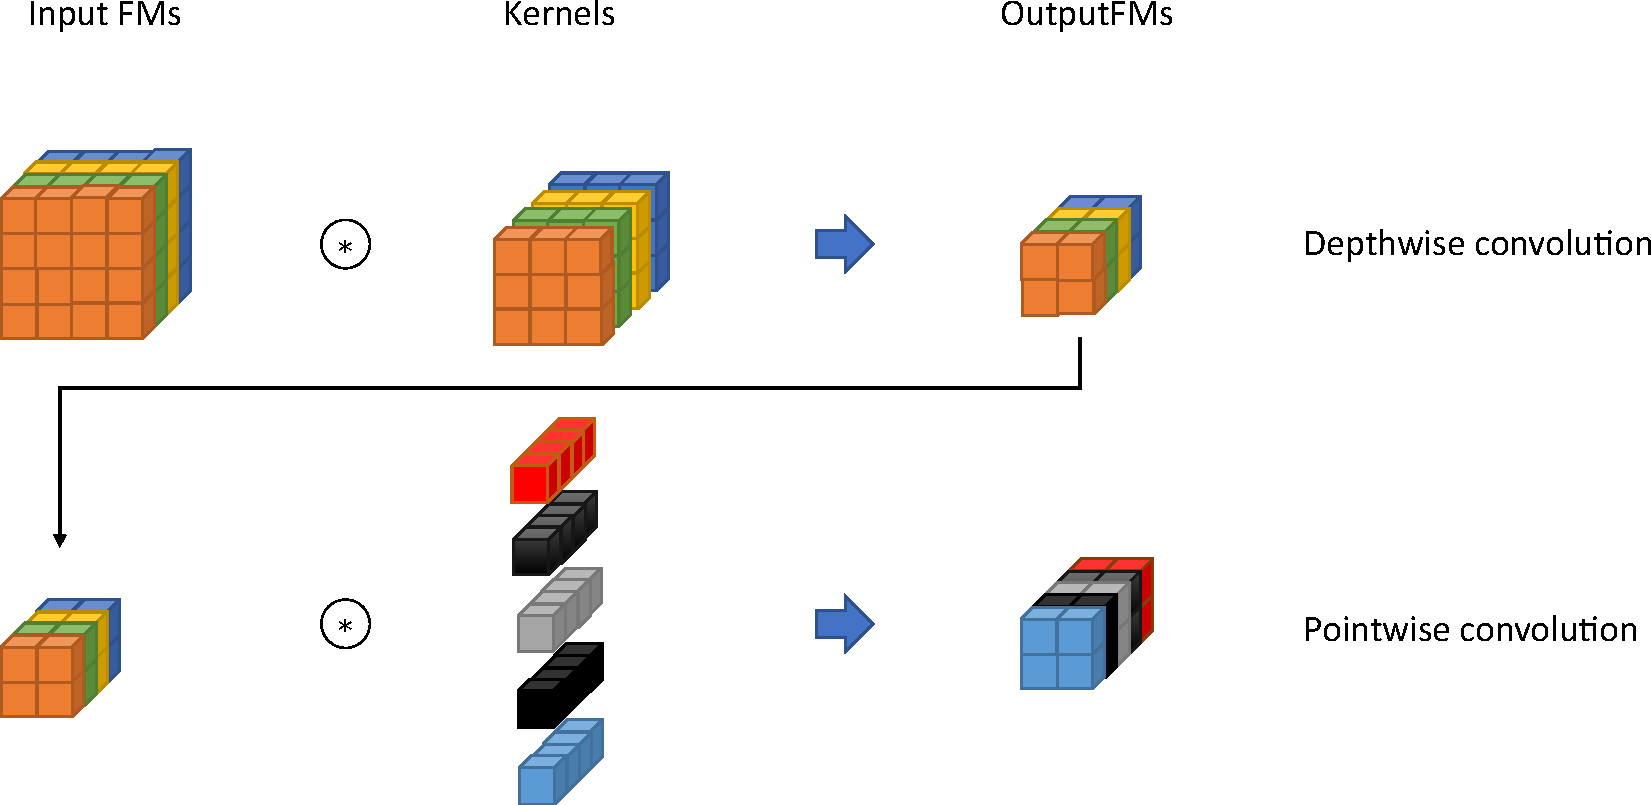
\includegraphics[width=\textwidth]{dsc.pdf}
    \caption{Depthwise Separable Convolution}
    \label{fig:dsc}
\end{figure}

%
\subsubsection{Pooling} \label{subs:pooling}
A Pooling layer is used to replace the output of the previous layer by a summary statistics of this output \cite{goodfellow_deep_2016}. They are usually inserted between the successive convolutional layer to modify the output further. Its goal is first to make the output approximately invariant to small translations and it also reduces the spatial size of each output \acrshort{fm}. It means that the memory needed to store the parameters is reduced \cite{goodfellow_deep_2016}. It also reduces the number of parameters and the computation of the network while also increasing the receptive field \cite{shawahna_fpga-based_2019}.

The pooling layer divides each \acrshort{fm} into regions of size $K \title K$ and outputs one pixel from each region. This way, is kept constant while their spatial size is reduced by $K$. Various pooling functions exist, but the most common form uses filters of size $2 \times 2$ where for example the MAX or AVG operation selects the highest pixel from 4 samples their average respectively (meaning a 75\% reduction of the pixels) \cite{suda_throughput-optimized_2016}. Figure \ref{fig:pool} illustrates an example of a pooling layer.
%
\begin{figure}
    \centering
    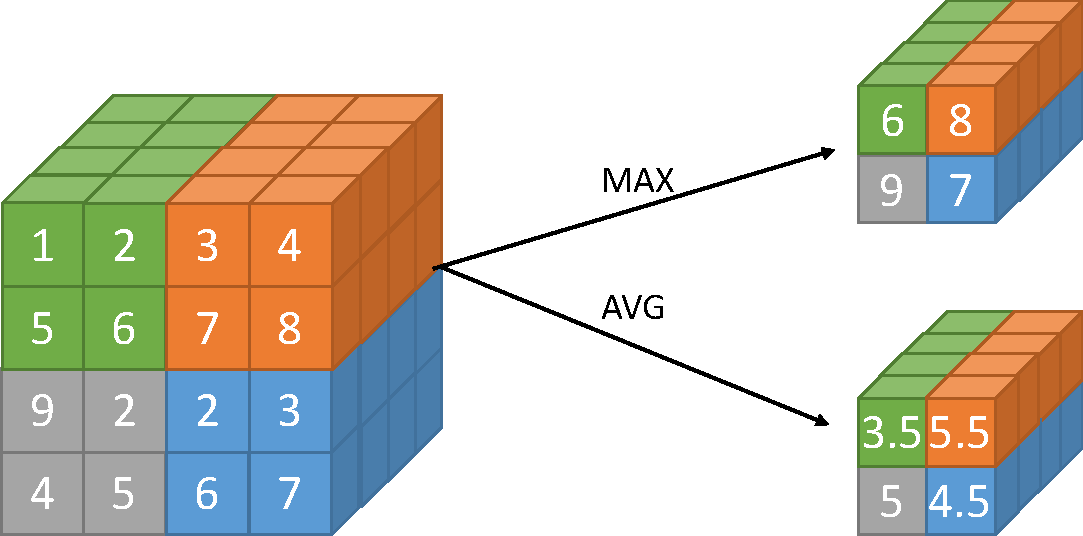
\includegraphics[width=0.8\textwidth]{pooling.pdf}
    \caption{An example of pooling layers}
    \label{fig:pool}
\end{figure}

%
%
\section{Training} \label{sec:train}
We have seen in the previous section what are the common building blocks in an \acrshort{cnn}. Now we explore how a network improves its performance, prediction, at a task automatically. This process is called "learning". Finding the correct methods to find the weights is then an important aspect to have an efficient network.

The learning phase starts after disigning the network. However, before the model can learn, we have to assign a value to the weight. The most common form is random initiliazation drawn from Gaussian distribution \cite{he_delving_2015}. The learning if affected by the initial values of the weight. If it is too small the network does not lear or if it is too large it might take a very long time to converge. To solve this, different initializations have been proposed: Xavier initiliazation \cite{glorot_understanding_2010} and He initialization \cite{he_delving_2015}.

Once the weights have been initialized, we can perform the backpropagation algorithm to improve the efficiency of the network. It is composed of two steps: the forward pass and the backward pass.
%
%
\subsubsection{Forward-propagation} \label{subs:trainforward}
%
The first step of the backpropagation algorithm is the forward propagation. During this step, the training data are used as input of the model and each input is propagated through the network using the initialized weights. A vector of outputs is produced and is compared using a loss function (for example mean-square error defined by Equation \eqref{eq:mse}) with the label of the input (target $\boldsymbol{t}$) \cite{matteucci_artificial_2019}. The weights are then adjusted in order minimize the loss function. This can be done using the algorithms found in the next section. When the model is trained, the inference consists only of the forward propagation \cite{abdelouahab_accelerating_2018}.
%
\begin{equation}
    L(\boldsymbol{x}, \boldsymbol{w}) = \sum^{N}_{i=1} (t_i - p(x_i, \boldsymbol{w}))^2
    \label{eq:mse}
\end{equation}

%
\subsection{Back-propagation} \label{subs:trainbackward}
According to \textcite{ruder_overview_2017}, gradient descent optimization algorithms are the most popular to perform optimizations on \acrshort{nn}. These algorithms derive from the idea of gradient descent. As said in the previous section, gradient descent is a way to minimize the loss function, parametrized by the model's parameters (weight). We can, therefore, describe gradient descent algorithm using equation \eqref{eq:gd}, where $\eta$ is the learning rate, a positive scalar determining the size of the step in the direction minimizing the gradient \cite{goodfellow_deep_2016}. If we update the weight in the opposite direction of the gradient, we can reach a local minimum.
%
\begin{equation}
    \boldsymbol{w} = \boldsymbol{w} - \eta \frac{ \partial L( \boldsymbol{x}, \boldsymbol{w} ) }{\partial \boldsymbol{w}}
    \label{eq:gd}
\end{equation}

\textbf{The original gradient descent} or \textbf{batch gradient descent }computes the gradient using the whole dataset (the batch). We see how to compute the gradient on equation \eqref{eq:gd-grad}. This might be impossible to do in practice if the dataset is too large. Variations have then be proposed to make the gradient descent to be practical.
%
\begin{equation}
    \frac{ \partial L( \boldsymbol{x}, \boldsymbol{w} ) }{\partial \boldsymbol{w}} = \frac{1}{Nin} \sum^{Nin}_{i = 0} \frac{ \partial L( x_i, \boldsymbol{w} ) }{\partial \boldsymbol{w}}
    \label{eq:gd-grad}
\end{equation}

\textbf{Stochastic gradient descent}, instead of using the entire dataset, performs the gradient descent algorithm on one sample at a time. We see how to compute the gradient on equation \eqref{eq:sgd-grad}. It avoids the redundant computation of the batch gradient descent. It learns faster and can reach better local minima, however, it is complicated to find the global minimum.
%
\begin{equation}
    \frac{ \partial L( \boldsymbol{x}, \boldsymbol{w} ) }{\partial \boldsymbol{w}} = \frac{ \partial L( x_i, \boldsymbol{w} ) }{\partial \boldsymbol{w}}
    \label{eq:sgd-grad}
\end{equation}

\textbf{Mini-batch gradient descent} is a trade-off between the two approaches. It performs an update of the weight for every mini-batch of $N$ training examples. It has better convergence  by reducing the variance and has less computation than batch gradient descent.
%
\begin{equation}
    \frac{ \partial L( \boldsymbol{x}, \boldsymbol{w} ) }{\partial \boldsymbol{w}} = \frac{1}{N} \sum^{N < Nin}_{i = 0} \frac{ \partial L( x_i, \boldsymbol{w} ) }{\partial \boldsymbol{w}}
    \label{eq:bgd-grad}
\end{equation}

%
%
\section{Models}
Once we have seen how to build and train a \acrshort{cnn}, we can now detail famous networks as example.
%
\subsubsection{AlexNet}
%
AlexNet is a famous \acrshort{cnn} which was developed in 2012 by \textcite{krizhevsky_imagenet_2012}. It is a breakthrough in the deep \acrshort{cnn} field and this model won the ImageNet competition. Krizhevsky et al. used some parameters optimizations and made the model deeper in order to considerably improve the learning ability of the CNN \cite{khan_survey_2020}. It is composed of 5 convolutional layers and 3 fully-connected layers, as seen in Figure \ref{fig:alexnet}. Each convolutional layer has a ReLU activation function and it uses pooling.
%
\begin{figure}[H]
    \centering
    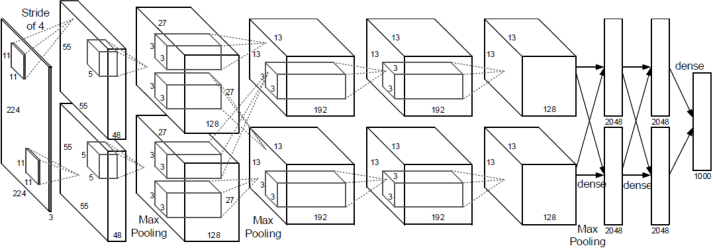
\includegraphics[width=\textwidth]{alexnet.pdf}
    \caption{An illustration of the architecture of AlexNet \cite{krizhevsky_imagenet_2012}}
    \label{fig:alexnet}
\end{figure}
%
\subsubsection{VGG}
%
After the success of AlexNet in 2012, research was made to reduce the computational complexity while keeping the accuracy. In 2014, VGG, a deeper variant of AlexNet was developed by \textcite{simonyan_very_2015}. It is composed of 5 groups of convolutional layers, where the number of layers depends on the version of VGG. It won the localization in the ImageNet challenge in 2014 \cite{simonyan_very_2015}. An illustration is provided by Figure \ref{fig:vgg}. This level of depth was possible thanks to the application of very small ($3 \times 3$) convolution kernels. They allow a larger receptive field with fewer parameters and more non-linearities than a larger kernel. However, it has a high memory request. 100MB per image needs to be stored in all \acrshort{fm}s for the forward propagation \cite{matteucci_artificial_2019}.
%
\begin{figure}[H]
    \centering
    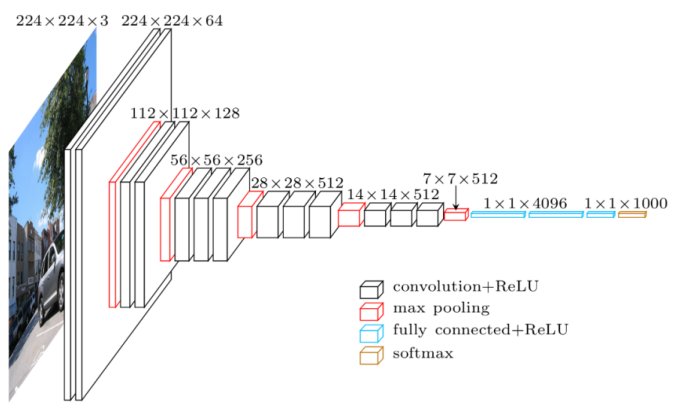
\includegraphics[width=0.75\textwidth]{VGG.pdf}
    \caption{An illustration of the architecture of VGG16 \cite{simonyan_very_2015}}
    \label{fig:vgg}
\end{figure}
%
\subsubsection{ResNet}
%
\textcite{he_deep_2016} developed ResNet in 2015. It is a very deep network which can contain from 50 to 1000 convolutional layers. It is composed of structures which are more complex and irregular than in the networks described previously. \textcite{he_deep_2016} showed that an increase of the depth of the network does not leads to an improvement of the performance. Indeed, beyond a certain amount of layers, a continuous increase of the depth leads to the degradation of the accuracy. This is not due to overfitting. It is because the deeper models are harder to optimize than shallower ones (vanishing gradient described in Section \ref{subs:trainbackward}) \cite{matteucci_artificial_2019}. 

However, deeper networks should at least have similar or better performance than shallower ones. Indeed, let’s compare a deeper and a shallower network. If the deeper network is composed of the same layers than the shallower one and that the other added layers are just identity mapping, then the network should have the same performance than the shallower one. Therefore, a deeper network should not have worse performance than shallower ones \cite{matteucci_artificial_2019}.

To overcome this issue, \textcite{he_deep_2016} introduced an \textit{identity shortcut connection} which skips one or more layers and set weights to the identity, as can be seen in Figure \ref{fig:resnet}. These weights associated to the shortcut connection can be used to learn a residual $\mathcal{F}(x)$ in order to improve the solution. The performance of this very deep network allowed it to win the 2015 ILSVR for both localization and classification.
%
\begin{figure}[H]
    \centering
    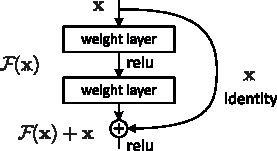
\includegraphics[width=0.7\textwidth]{resnet.pdf}
    \caption{ResNet building block, from \cite{he_deep_2016}}
    \label{fig:resnet}
\end{figure}
%
\subsubsection{MobileNetV2} \label{subs:mbv2}
%
According to \textcite{cheng_recent_2018}, the performance of \acrshort{cnn} in recent years became outstanding. These improvements came at the cost of storage and computational complexity. It is not an issue for the \acrshort{cnn} training phase, because the GPU and CPU also gained in computational units and memory. However, for the inference phase, the computational complexity and the storage requirements are way beyond the capabilities of most of the embedded applications and mobile devices such \acrshort{fpga} \cite{cheng_recent_2018}.
%
\begin{itemize}
    \item The enormous computational complexity of \acrshort{cnn}s makes it difficult to deploy on real-time applications and it consumes battery power.
    \item The large number of parameters of \acrshort{cnn}s consumes considerable storage and run-time memory.
\end{itemize}

In order to overcome this issue, \textcite{sandler_mobilenetv2_2018} introduced a network called MobileNetV2 in 2018. It is specifically developed for constrained environments. First, the size and number of operations is decreased thanks to DSC (see Section \ref{subs:dsc}) and thanks to a new type of layer \textit{inverted residual with a linear bottleneck}, which can be observed in Figure \ref{fig:invreslinbot} and Table \ref{tab:invreslinbot}.
This layer is composed of a $1 \times 1$ convolution to expand the number of the input \acrshort{fm} channels by a factor $t$ ($N_{intf} = t \times N_{if}$). It is then followed by a \acrshort{dsc}. The purpose of the first convolution layer which increases the number of channels is supposed to counterbalance the loss of information that occurred by the ReLU activation. They also added a skip connection to build a network of great depth, and the last convolution has a linear activation function \cite{sandler_mobilenetv2_2018}.
%
\begin{figure}[H]
    \centering
    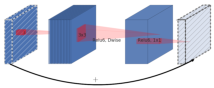
\includegraphics[width=\textwidth]{mbnv2.pdf}
    \caption{inverted residual with linear bottleneck \cite{sandler_mobilenetv2_2018}}
    \label{fig:invreslinbot}
\end{figure}
%
\begin{table}
    \center
    \begin{tabular}{c|c|c}
        Input & Operetor & Output \\
        \hline \hline
        $N_{ix} \times N_{iy} \times N_{if}$ & $1 \times 1$ conv2d, ReLU6 & $N_{ix} \times N_{iy} \times (t \times N_{if})$ \\
        $N_{ix} \times N_{iy} \times (t \times N_{if})$ & $3 \times3$ dwise s=$s$, ReLU6 & $\frac{N_{ix}}{s} \times \frac{N_{iy}}{s} \times (t \times N_{if})$ \\
        $\frac{N_{ix}}{s} \times \frac{N_{iy}}{s} \times (t \times N_{if})$ & $1 \times 1$ conv2d & $\frac{N_{ix}}{s} \times \frac{N_{iy}}{s} \times N_{of}$ \\
        \hline \hline
    \end{tabular}
    \caption{inverted residual with linear bottleneck \cite{sandler_mobilenetv2_2018}}
    \label{tab:invreslinbot}
\end{table}

More information about the structure of MobileNetV2 can be found in Appendix \ref{appendix:mbv2}.

%
%
\section{Optimizations}
%
%
In this section, we explore the state-of-the-art approaches to reduce the arithmetic complexity and the hardware utilization of \acrshort{cnn} models. Section \ref{subsec:algopti} details how to efficiently handle and optimize the convolution operation on \acrshort{fpga}. On the other side, section \ref{subsec:mdopti} goes over techniques to reduce the size of the model.
%
\section{Algorithmic Optimizations} \label{sec:algopti}
In this section we will review algorithmic optimization techniques to reduce computational complexity of convolutions, which are a costly operation. According to \cite{shawahna_fpga-based_2019}, 90\% of computation time in \acrshort{cnn} are consummed by the convolution operation.
%
%
\subsection{\acrfull{gemm}}
%
%
It is a common way to process \acrshort{cnn} on \acrshort{cpu} and \acrshort{gpu}. We convert the convolution as a matrix-vector multiplication.  The process of a convolution layer can be observed on Figure \ref{fig:gemm}.
However, this approach is not suggested for \acrshort{fpga}: \cite{sze_efficient_2017, zhu_efficient_2020} point out that the \acrshort{fm}s have to be copied multiple times when flattened to a vector. It leads to a huge memory footprint and either ineffiency in storage or complex memory management access patterns.
\begin{figure}
    \centering
    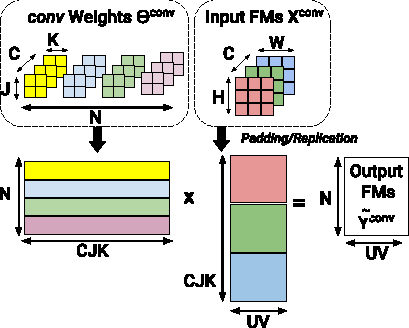
\includegraphics[width=0.5\textwidth]{Images/gemm.pdf}
    \caption{\acrshort{gemm} base processing on conv layer}
    \label{fig:gemm}
\end{figure}
%
%
\subsection{Winograd Transform}
%
%
The Winograd minimal filter algorithm is first introduced by \cite{winograd_arithmetic_1980}. We can apply this computational transform to convolutions when the stride is equal to 1. In Winograd filtering, data is processed by blocs referred as \textit{tiles}, as following:
\begin{itemize}
    \item An input \acrshort{fm} tile $g$ of size $(N_{ix} \times N_{iy})$ is pre-processed: $\tilde{g} = \boldsymbol{G^{T}} g \boldsymbol{G} $, where $\boldsymbol{G}$ is a transformation matrix defined in the Winograd Algorithm \cite{winograd_arithmetic_1980}.
    \item In a same way, $d$, the filter of size $(K_x \times K_y)$ is transformed into $\tilde{d}$: $\tilde{d} = \boldsymbol{B^{T}} d \boldsymbol{B}$ , where $\boldsymbol{B}$ is a transformation matrix defined in the Winograd Algorithm \cite{winograd_arithmetic_1980}.
    \item The output tile $Y$ of the Winograd Filtering algorithm, denoted $F(N_{ix} \times N_{iy}, K_x \times K_y)$ is computed using equation \ref{eqn:winograd}, where $\boldsymbol{A}$ is a transformation matrix defined in the Winograd Algorithm \cite{winograd_arithmetic_1980} and $\odot$ indicates element-wise multiplication.
\end{itemize}
\begin{equation}
\label{eqn:winograd}
Y = \boldsymbol{A^{T}} [ \ \tilde{g} \odot \tilde{d} \ ] \boldsymbol{A}
\end{equation}
\cite{lavin_fast_2015} demonstrated that Winograd convolution is efficient when the kernel is small ($K_* \leq 3$) and the number of multiplication can be reduced by a factor of $2.25 \times$ (in returns the number of addition is increased). According to \cite{sandler_mobilenetv2_2019}, $3 \times 3$ kernel is a standard for modern networks, which leads to think that Winograd Transform is a usefull approach to reduce computational complexity of convolutional layers. For example, \cite{aydonat_opencl_2017, lu_evaluating_2017} utilized Winograd transform and haved reduced their computational complexity by around 50\%.
%
%
\subsection{\acrfull{fft}}
%
%
The \acrshort{fft} is an algorithm to transform the 2D convolution into element-wise multiplication in the frequency domain. The equation is observed at equation \ref{eqn:fft}
\begin{equation}
\label{eqn:fft}
conv2D(FM_{I}[ic], K[oc, ic]) = IFFT( FFT(FM_{I}[ic]) \odot FFT(K[oc, ic]) )
\end{equation}
The arithmetic complexity of the 2D convolution can be reduced to $O(N_{ix}^2 log_2(N_{ix}))$ \cite{jong_hwan_ko_design_2017} and the computational complexity of the \acrshort{fft} can be reduced to $O(N_{ix} log_2(K_{x}))$ using the Overlap-and-Add Method \cite{w_smith_scientist_1997}.
However, the \acrshort{fft} finds its interest when kernel are large \cite{lavin_fast_2015} ($K_* \geq 5$), which is not a standard kernel size according to \cite{sandler_mobilenetv2_2019}. \cite{zhang_frequency_2017} implemented \acrshort{fft} algorithm for \acrshort{cnn} on \acrshort{fpga} and it showed little reduction of computation complexity with small filters such as $3 \times 3$.

%
\subsection{Model Optimizations} \label{subsec:mdopti}
As mentioned previously, the major issues, when implementing a \acrshort{cnn} on an \acrshort{fpga}, are the \acrshort{cnn} size and its computational complexity. Research was done to develop techniques tackling those two issues by directly modifying the \acrshort{cnn} architecture. \textcite{nurvitadhi_can_2017} believe that sparsity exploitation and extremely compact data types will become the norm in next-generation \acrshort{cnn}s.
%
%
\subsubsection{Efficient Model Design}
%
Section \ref{subsec:models} presented several state-of-the-art models. However, those models (except MobileNetV2) were designed to provide the highest performance possible but did not consider the implementation of such models on mobile and embedded devices \cite{iandola_squeezenet_2016}. Therefore, several other models were designed to run on such constrained platforms trading a reduction of the number of parameters and operations in exchange for a drop of accuracy. Indeed, if we observe Figure \ref{fig:archi}, the lightweight models do not match the high-performance ones in terms of accuracy only.

A clever choice of design decreases the number of parameters and computations of the model while reducing the drop of accuracy. As many approaches were proposed to reduce the size of a model, this study will focus on architectures that target the embedded space. This section describes five of these architectures:
\begin{itemize}
    \item \textbf{SqueezeNet} \cite{iandola_squeezenet_2016} was focused on reducing the number of parameters of AlexNet (see Section \ref{subsec:models}) by introducing a new building block: \textbf{Fire Module}. Therefore, their architectures are very similar. SqueezeNet replaces all layers (except the first and last one) by \textbf{Fire Modules}. The \textbf{Fire Module}, observed in Figure \ref{fig:archi_building_block:sqn}, is composed of two convolutional layers. The first one called \textit{squeeze block} only performs $1 \times 1$ convolutions to squeeze the number of input channels. The reduction of the number of channels decreases the computational complexity and number of parameters of the next convolutional layer. Moreover, they also chose $1 \times 1$ convolution because it requires fewer parameters than $3 \times 3$ convolution.
    The second convolutional layer called \textit{expand block} is composed of $1 \times 1$ and $3 \times 3$ convolutions. With this architecture, the size of AlexNet is decreased from $240$MB to $4.8$MB \cite{iandola_squeezenet_2016}. It can even be reduced to $0.47$MB without a drop in accuracy method by applying Deep Compression \cite{han_deep_2016}. However, it has a big memory footprint, is slower in runtime, and consumes more energy than AlexNet \cite{sze_efficient_2017}.
    %
    \item \textbf{MobileNet} \cite{howard_mobilenets_2017} uses \acrshort{dsc}, described in Section \ref{subs:dsc}, to build small and low latency models that can fulfill the design requirements, as can be seen in Figure \ref{fig:archi_building_block:mbn}. Two hyper-parameters are used to set the model size and throughput:
    %
    \begin{itemize}
        \item The width multiplier $\alpha \in [1; 0[$, which reduces the number of input and output channels at each layer,
        \item The resolution multiplier $\rho \in [1; 0[$,  which reduces spatially the input and output \acrshort{fm}s at each layer.
    \end{itemize}
    %
    \item \textbf{ShuffleNet}  was developed by \textcite{zhang_shufflenet_2018}, in 2018. It is designed to be a computation efficient architecture, especially for mobile devices with very limited computing power. Indeed, it reduces the computation cost while maintaining the accuracy by using \textbf{pointwise group convolution}, decreasing the computation complexity of $1 \times 1$ convolutions. It also uses \textbf{channel shuffle} operation on the channels such that \textbf{group convolutions} obtain information from different groups. Then more powerful structures can be built with multiple group convolutional layers. However, the group convolutions and the bottleneck structures add \acrfull{mac} which is a non-negligible cost \cite{ma_shufflenet_2018}. The group convolution contributes to network fragmentation and reduces parallelism. Moreover, the \textquote{Add} operation, as seen in Figure \ref{fig:archi_building_block:shn}, is quite significant.
    %,
    \item \textbf{NasNet} was developed by \textcite{zoph_learning_2018}, in 2018. The idea was to use a search method called \acrfull{nas}, to find good convolutional architectures on a specific dataset. For that purpose, NasNet uses a \acrfull{rnn} to generate efficient architectures. The \acrshort{rnn} generates sample child networks with different architectures, which are trained to convergence. The accuracy of the child networks is used to train the \acrshort{rnn}, which will generate better architectures over time. A convolution layer can be seen in Figure \ref{fig:archi_building_block:nasn}. The learned architecture is flexible as it may be scaled in terms of computational cost. The network provides a higher accuracy with comparable parameters and \acrshort{mac} than MobileNet and ShuffleNet (described previously) \cite{zoph_learning_2018}. However, the resulting network ends up very complex \cite{sandler_mobilenetv2_2018}.
    %
    \item \textbf{MobileNetV2} was developed by \textcite{sandler_mobilenetv2_2018}, in 2018. It is an improvement of MobileNet (described previously) in terms of accuracy and does not require special operators. It has also a smaller memory footprint. Furthermore, MobileNetV2 has faster inference and fewer parameters than MobileNet. MobileNetV2 has already been explained in Section \ref{subs:mbv2}.
\end{itemize}
%
\begin{figure}[H]
    \centering
    %
    \begin{subfigure}[t]{0.49\linewidth}
        \centering
        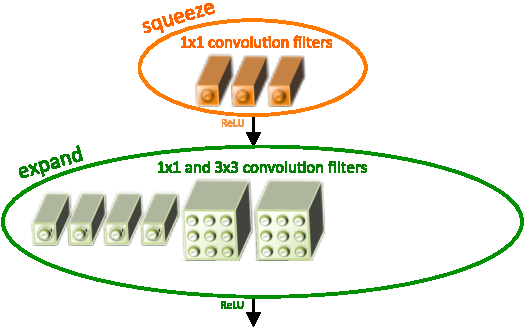
\includegraphics[width=\textwidth, height=0.3\textheight, keepaspectratio]{squeeze.pdf}
        \caption{Squeezenet Fire Module\cite{iandola_squeezenet_2016}}
        \label{fig:archi_building_block:sqn}
    \end{subfigure}
    %
    \begin{subfigure}[t]{0.49\linewidth}
        \centering
        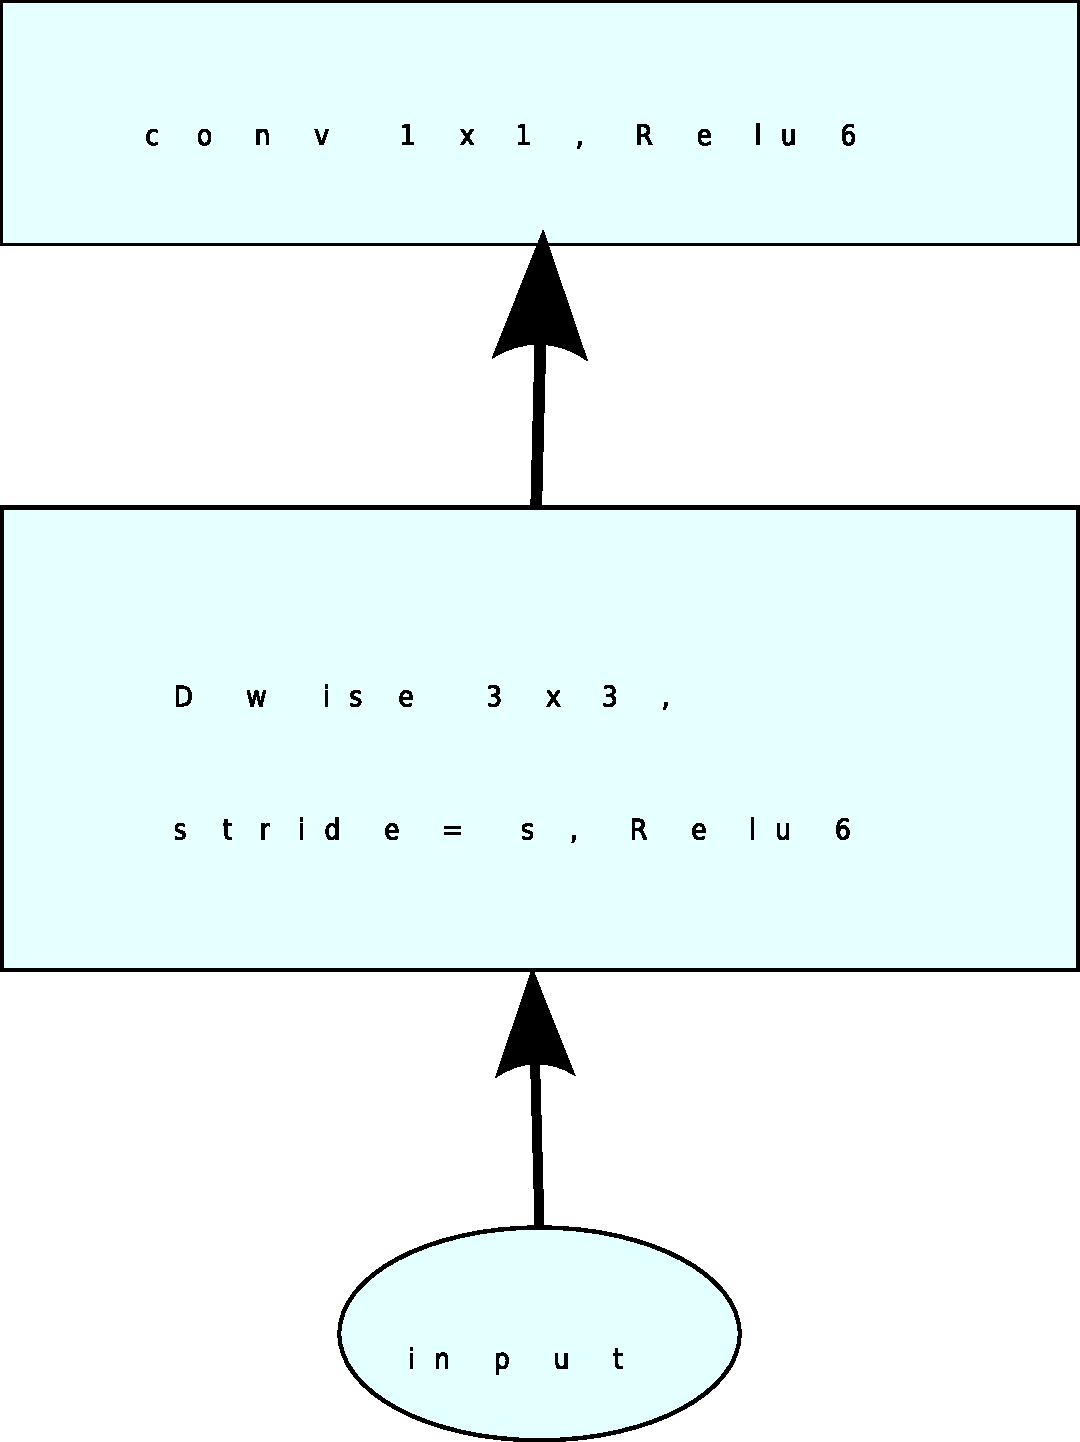
\includegraphics[width=\textwidth, height=0.2\textheight, keepaspectratio]{mobilenet.pdf}
        \caption{MobileNet convolutional block \cite{howard_mobilenets_2017}}
        \label{fig:archi_building_block:mbn}
    \end{subfigure}
    %
    \begin{subfigure}[t]{0.49\linewidth}
        \centering
        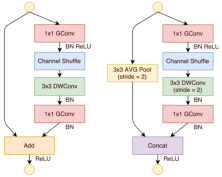
\includegraphics[width=\textwidth, height=0.2\textheight, keepaspectratio]{shufflenet.pdf}
        \caption{ShuffleNet convolutional block \cite{zhang_shufflenet_2018}}
        \label{fig:archi_building_block:shn}
    \end{subfigure}
    %
    \begin{subfigure}[t]{0.49\linewidth}
        \centering
        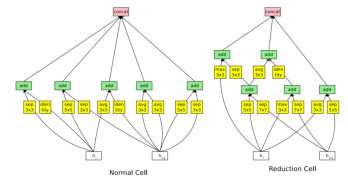
\includegraphics[width=\textwidth, height=0.3\textheight, keepaspectratio]{nasnet.pdf}
        \caption{NasNet convolutional blocks \cite{zoph_learning_2018}}
        \label{fig:archi_building_block:nasn}
    \end{subfigure}
    %
    \begin{subfigure}[t]{0.49\linewidth}
        \centering
        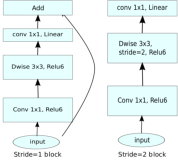
\includegraphics[width=\textwidth, height=0.2\textheight, keepaspectratio]{mobilenet2.pdf}
        \caption{MobileNetv2 convolutional blocks \cite{sandler_mobilenetv2_2018}}
        \label{fig:archi_building_block:mb2n}
    \end{subfigure}
    %
    \caption{Convolutional block from different architectures}
    \label{fig:archi_building_block}
\end{figure}

The architecture used in this work was developed to implement MobileNetV2 because of its simplicity and its state-of-the-art performance (see Table \ref{tab:mbv2}). Moreover, MobileNetV2 requires fewer parameters while providing state-of-the-art accuracy when comparing to the different architectures, as shown in Figure \ref{fig:archi}.
%
\begin{table}[H]
    \center
    \begin{tabular}{ | c | c | c c | c| }
        \hline \hline
        Network & Top 1 & Params & MAdds & CPU \\
        \hline \hline
        MobileNetV1 & 70.6 & 4.2M & 575M & 113ms \\
        ShuffleNet (1.5) & 71.5 & \textbf{3.4M} & 292M & - \\
        ShuffleNet (x2)  & 73.7 & 5.4M & 524M & - \\
        NasNet-A & 74.0 & 5.3M & 564M & 183ms \\
        \hline
        MobileNetV2 & \textbf{72.0} & \textbf{3.4M} & \textbf{300M} & \textbf{75ms} \\
        MobileNetV2 (1.4) & \textbf{74.7} & 6.9M & 585M & \textbf{143ms} \\
        \hline \hline
    \end{tabular}
    \caption{Performance on ImageNet, comparison for different networks \cite{sandler_mobilenetv2_2018}}
    \label{tab:mbv2}
\end{table}

\begin{figure}[H]
    \centering
    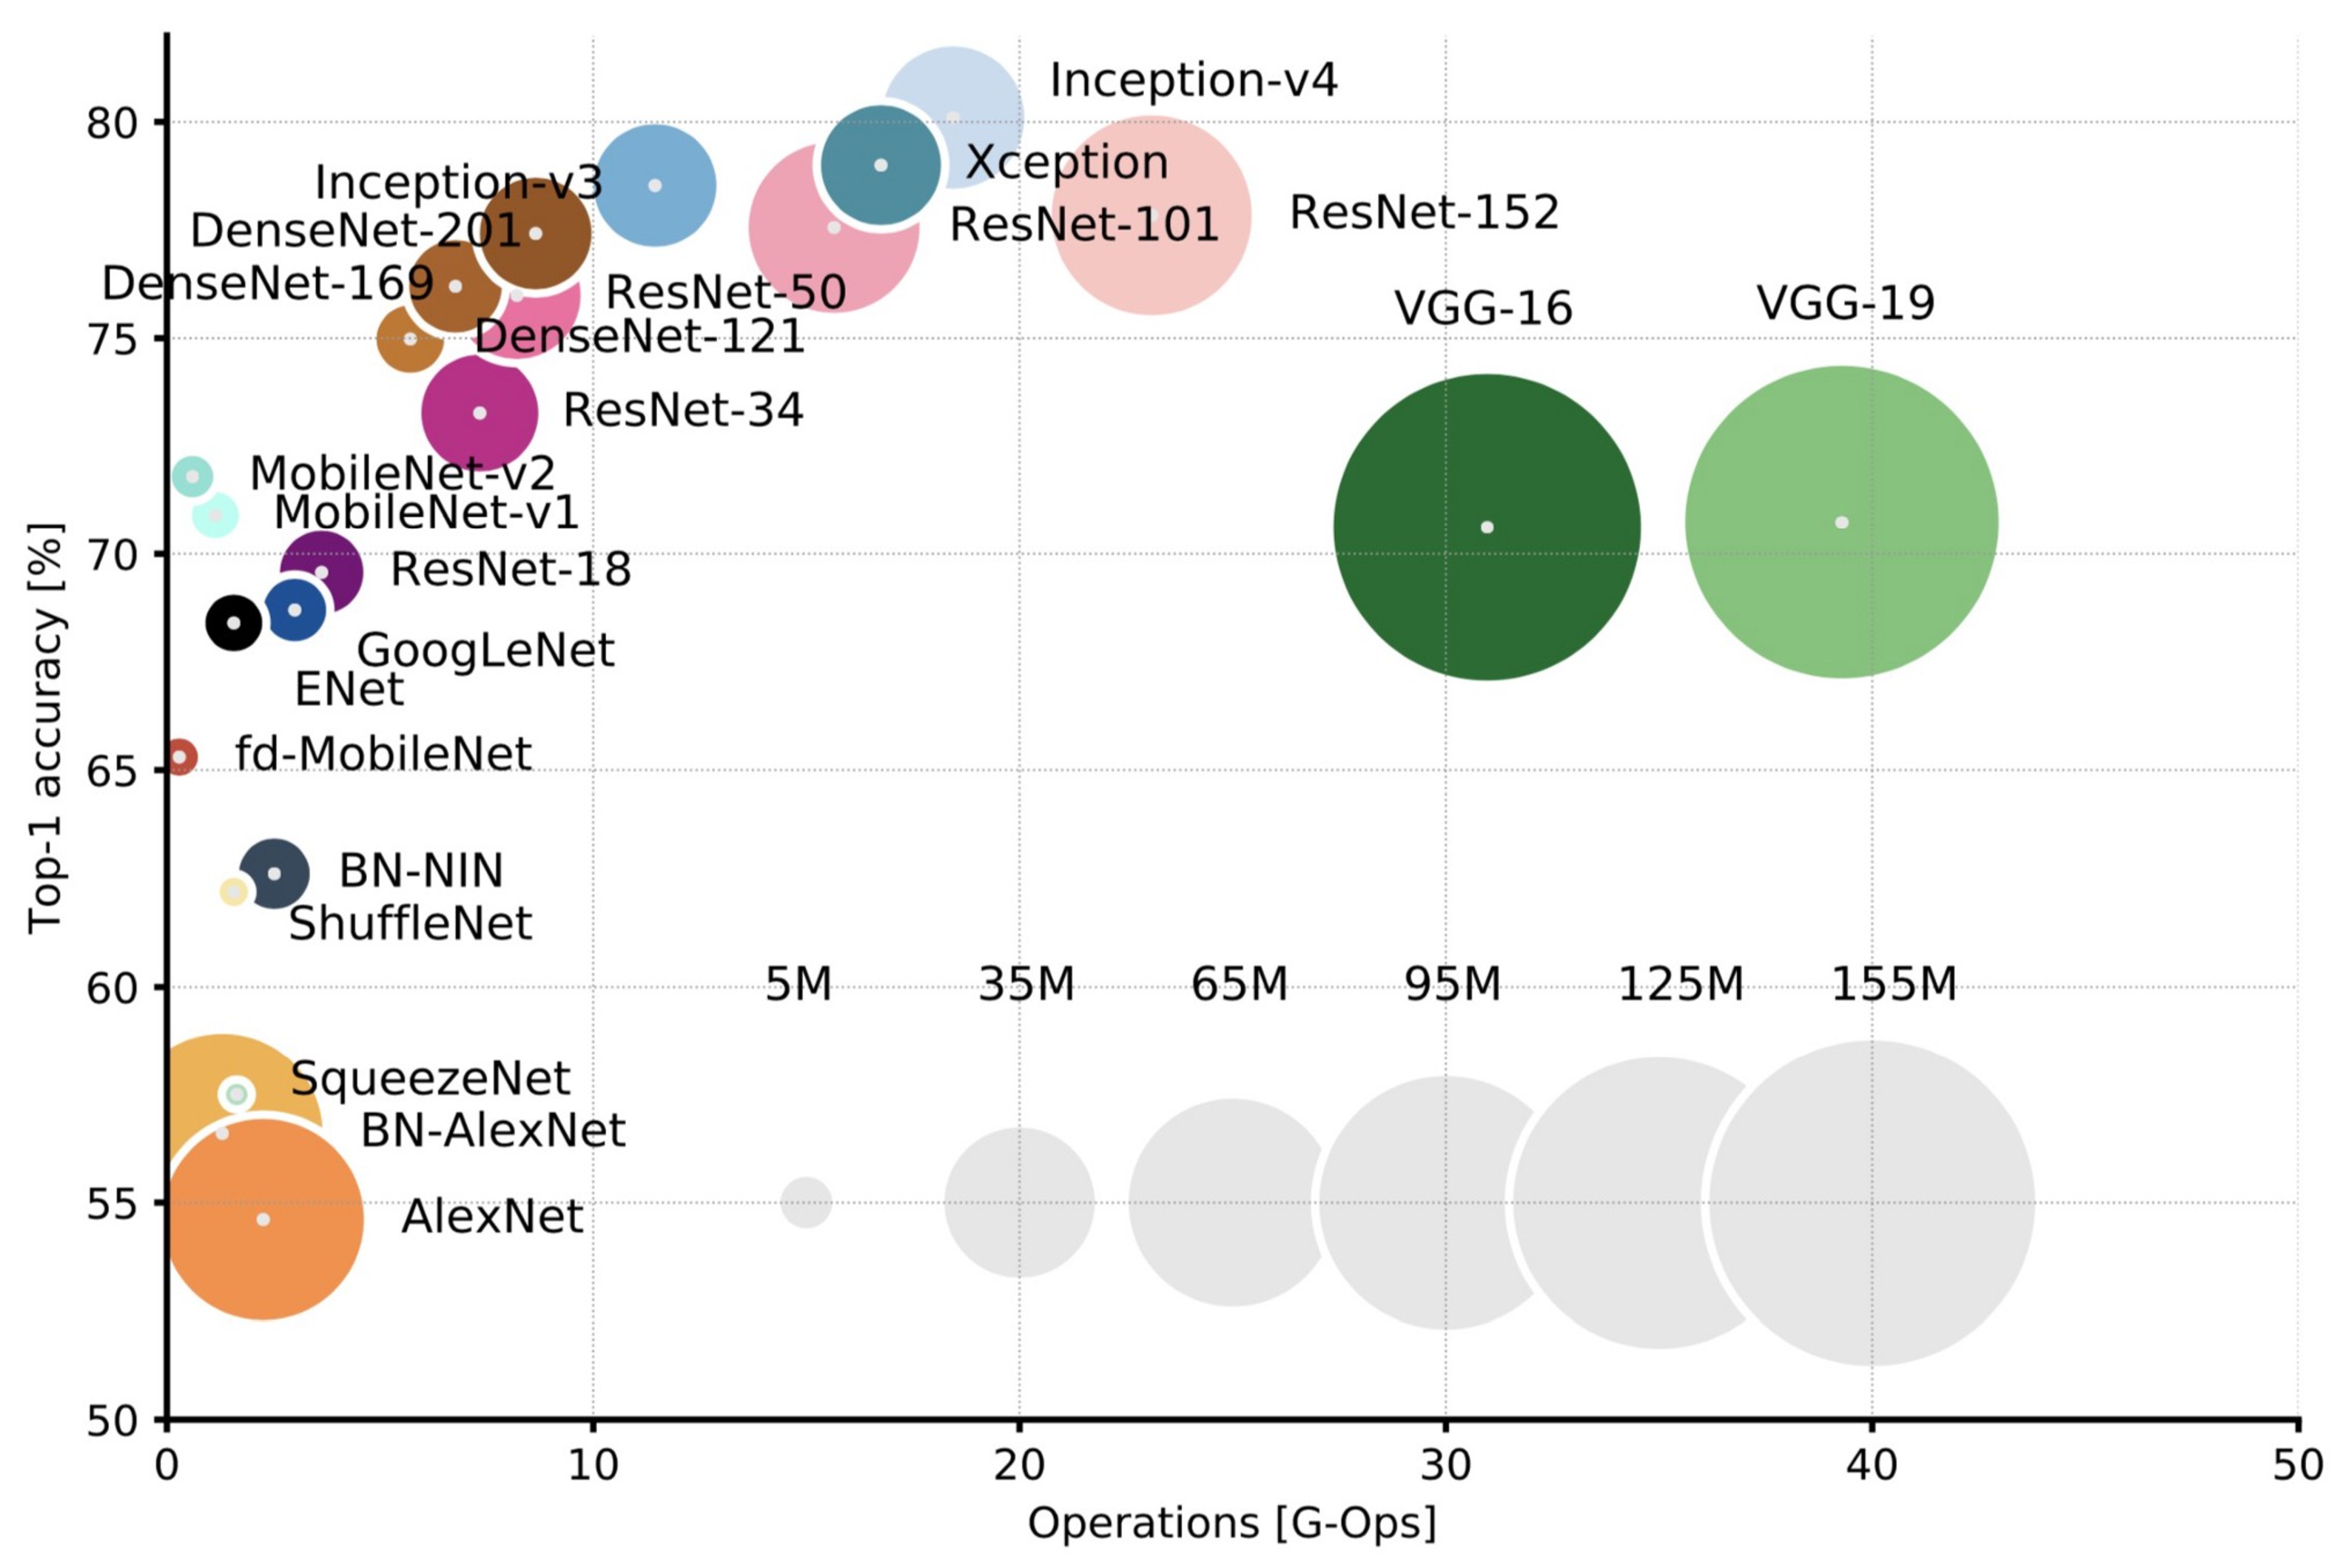
\includegraphics[width=0.9\textwidth]{archi.pdf}
    \caption{Ball chart reporting the Top-1 accuracy of various architectures vs. their computational complexity \cite{canziani_analysis_2017}}
    \label{fig:archi}
\end{figure}
%
\subsubsection{Pruning} \label{subs:pruning}
%
To improve the inference phase of a \acrshort{cnn}, pruning can be used, especially for platforms with limited computational resources \cite{liu_rethinking_2019}. According to \textcite{liu_rethinking_2019, denton_exploiting_2014}, the huge number of parameters in a network might create a problem of \textbf{over-parametrization}. Over-parametrization means that there are redundancies in \acrshort{nn} parameters and that the same performance could be achieved with only a subset of them. In other words, a lot of parameters are unimportant or unnecessary \cite{cheng_recent_2018}. Pruning is defined as removing the parameters considered as not important. For example, \textcite{baoyuan_liu_sparse_2015} achieve more than 90\% sparsity of parameters in convolutional layers in AlexNet with less than 1\% accuracy loss.

We can explain why pruning works by \textbf{The Lottery Ticket Hypothesis} \cite{frankle_lottery_2018, frankle_early_2020}: \textquote{\textit{A randomly initialized, dense neural network contains a subnetwork that is initialized such that—when trained in isolation—it can match the test accuracy of the original network after training for at most the same number of iterations.}} From this postulate, those unimportant weights can be set to zero (prune) because they do not improve the accuracy of the model.

According to \textcite{cheng_recent_2018}, pruning has two major benefits for the inference phase. First, less storage is required. Indeed, the non-pruned weights are sparsely distributed among the kernels. Thus, they can be stored in a compressed format reducing memory utilization. Second, pruning reduces the arithmetic complexity of the network. As convolutions perform a weighted sum with the input \acrshort{fm}, each \acrfull{mac} operation with a pruned weight can be discarded. Moreover, \textcite{han_learning_2015, mao_exploring_2017, kang_accelerator-aware_2020} pointed out that some pruning ratios can also improve the accuracy of the network, which can be explained by a form of regularization.

Various pruning schemes are focused on increasing the sparsity of the network without a drop of accuracy \cite{han_deep_2016, han_learning_2015}.  We call this pruning scheme where all unimportant parameters are pruned without extra constraint \textbf{unstructured pruning} \cite{cheng_recent_2018}. However, it is challenging to exploit the performance and the high parallelism of \acrshort{fpga} with this kind of pruned network. Indeed, this kind of pruning scheme creates irregularities in the data access pattern \cite{zhu_efficient_2020}. It means that the number of pruned weights is different in each kernel, and we should adapt the circuitry to the worst case. As a consequence, all filters conduct wasteful operations except the worst case \cite{shimoda_filter-wise_2019}. Furthermore, \textcite{anwar_structured_2017} pointed out that unstructured pruning requires overhead for computing addresses of the sparse non-pruned elements. Therefore, we should find pruning patterns that would be more hardware-friendly.

In contrast to the unstructured pruning, we have \textbf{structured pruning} schemes \cite{kang_accelerator-aware_2020}. They combine a structure regularization for accuracy and locality optimization for computation efficiency. According to \textcite{anwar_structured_2017}, \textquote{\textit{Structured pruning has no or little extra costs}}. We can categorize the various schemes into different groups \cite{cheng_recent_2018, kang_accelerator-aware_2020, anwar_structured_2017, wen_learning_2016}:
\begin{itemize}
    \item \textbf{Depth-wise}: all the weights of a layer are pruned. The layer is then removed.
    \item \textbf{Kernel-wise}: instead of pruning all the weights, we keep a ratio of kernels, which means a reduction of the number of output channels. This pruning scheme is provided in Figure \ref{fig:struct_pruning:fw}.
    \item \textbf{Channel-wise}: it is one of the most popular methods because it still can fit in the convolutional deep learning frameworks \cite{liu_rethinking_2019}. A layer of the input \acrshort{fm} is pruned, which means that the layer is also pruned in all the kernels, as can be seen in Figure \ref{fig:struct_pruning:chw}.
    \item \textbf{Shape-wise}: we prune the same weights in each kernel or group of kernels. For example, this pruning scheme was used in \textcite{zhu_efficient_2020}. It is illustrated in Figure \ref{fig:struct_pruning:sw}
\end{itemize}
%
\begin{figure}[H]
    \centering
    %
    \begin{subfigure}[t]{.32\textwidth}
    \centering
    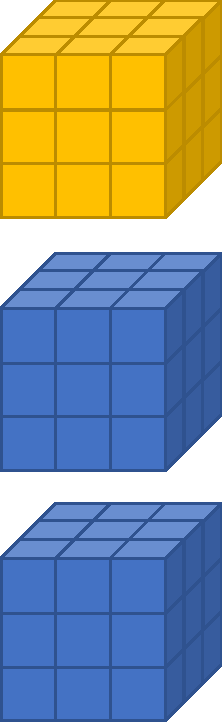
\includegraphics[width=0.33\linewidth]{filterwise.pdf}
    \caption{kernel-wise pruning}
    \label{fig:struct_pruning:fw}
    \end{subfigure}
    %
    \begin{subfigure}[t]{.32\textwidth}
    \centering
    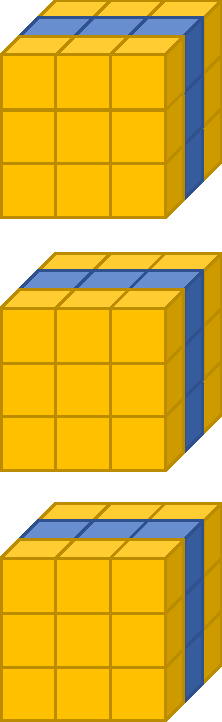
\includegraphics[width=0.33\linewidth]{channelwise.pdf}
    \caption{channel-wise pruning}
    \label{fig:struct_pruning:chw}
    \end{subfigure}
    %
    \begin{subfigure}[t]{.32\textwidth}
    \centering
    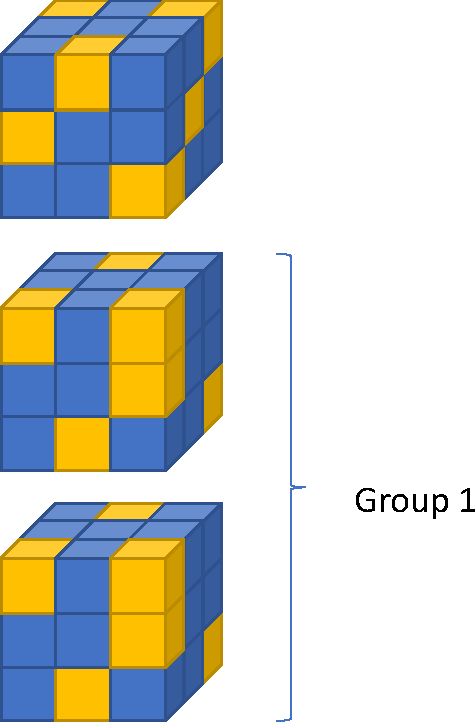
\includegraphics[width=0.70\linewidth]{shapewise.pdf}
    \caption{shape-wise pruning}
    \label{fig:struct_pruning:sw}
    \end{subfigure}
    %
    \caption{Structured pruning schemes, where the yellow weights are the pruned ones, inspired by \cite{cheng_recent_2018}}
    \label{fig:struct_pruning}
\end{figure}
%
The previously cited pruning schemes are ordered from very coarse-grained to fine-grained sparsity \cite{mao_exploring_2017}. As explained previously, coarse-grained sparsity (channel-wise and filter-wise pruning) provides a higher acceleration and can be used when implementing \acrshort{cnn} on \acrshort{gpu} or \acrshort{cpu} \cite{cheng_recent_2018, mao_exploring_2017}. However, finer-grained ones provide higher accuracy and as the sparsity increases, the accuracy is less affected, as can be seen in Figure \ref{fig:pruning-accuracy}. Therefore, this work focuses on developing customized hardware that can exploit a more fine-grained sparsity \cite{mao_exploring_2017} to provide a higher pruning while limiting the drop of accuracy.
%
\begin{figure}[H]
    \centering
    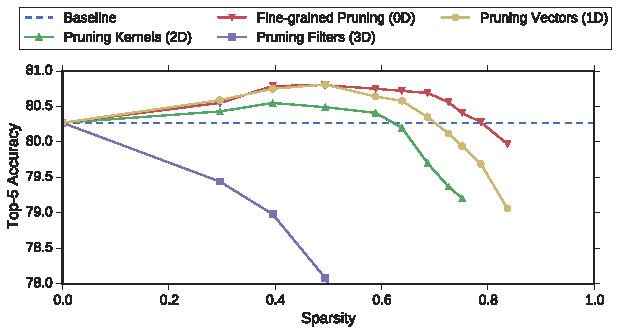
\includegraphics[width=\textwidth]{accuracysparsity.pdf}
    \caption{Accuracy-Sparsity Curve of AlexNet obtained by pruning \cite{mao_exploring_2017}}
    \label{fig:pruning-accuracy}
\end{figure}
%
Some studies focused on the acceleration of the inference step of lightweight models thanks to pruning. \textcite{zhang_channel_2019, tu_pruning_2019} applied pruning on \acrshort{dsc} kernels. They both chose \textbf{Channel-wise} pruning because it does not create sparse connections and it efficiently improves the speed of the inference. It also reduces the computational cost of the $1 \times 1$ (pointwise) convolutions, which has the biggest number of parameters and computational complexity. In MobileNet, it is about 95\%. By discarding one channel, the associated depthwise convolution is also avoided.
Moreover, the pointwise kernel producing that channel in the previous block can also be pruned. We can see the process in Figure \ref{fig:pruning_dsc}.
%
\begin{figure}[H]
    \centering
    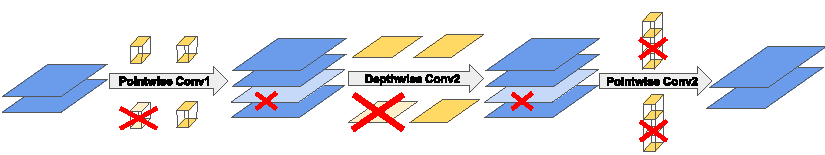
\includegraphics[width=\textwidth]{channelwise_ex.pdf}
    \caption{Pruning a depthwise separable convolution \cite{tu_pruning_2019}}
    \label{fig:pruning_dsc}
\end{figure}

\textbf{In this work, we focus on a structured pruning scheme for depthwise separable convolution. More precisely, we develop an architecture on \acrshort{fpga} than combines both advantages of pruning and depthwise separable convolution.}
%
\subsubsection{Quantization} \label{subs:quantization}
%
%
Quantization is an approach to trade accuracy for a decrease of the storage requirements of a network \cite{han_deep_2016}. Indeed, we can define quantization as the reduction of the number of bits representing a weight or pixel. Moreover, instead of using a floating-point number, we can use a \textbf{fixed-point number} \cite{cheng_recent_2018}. As said previously, fixed-point numbers are known to be more efficient on hardware such as \acrshort{fpga} because we can use integer arithmetic \cite{david_hardware_2007}. Quantization to fixed-point numbers can then reduce the memory requirement and the latency of the inference stage.

The format to encode the fixed-point representation of a real number is the \textit{Q-format} \cite{ward_real-time_2001}. A N-bit number, noted $Q_{m.n}$, is divided into two parts separated by an implied binary point. The $m$ bits are used to represent the integer part of the number (including the sign bit), and the $n$ bits are used to represent the fractional part, as can be seen in Figure \ref{fig:Qformat}. The bitwidth associated with each part can be either the same, either fine-tuned for each layer after analysis. Indeed, \textcite{qiu_going_2016, yin_high_2018} choose a different range for each layer, but doing it for every weight is not memory-efficient.
%
\begin{figure}[H]
    \centering
    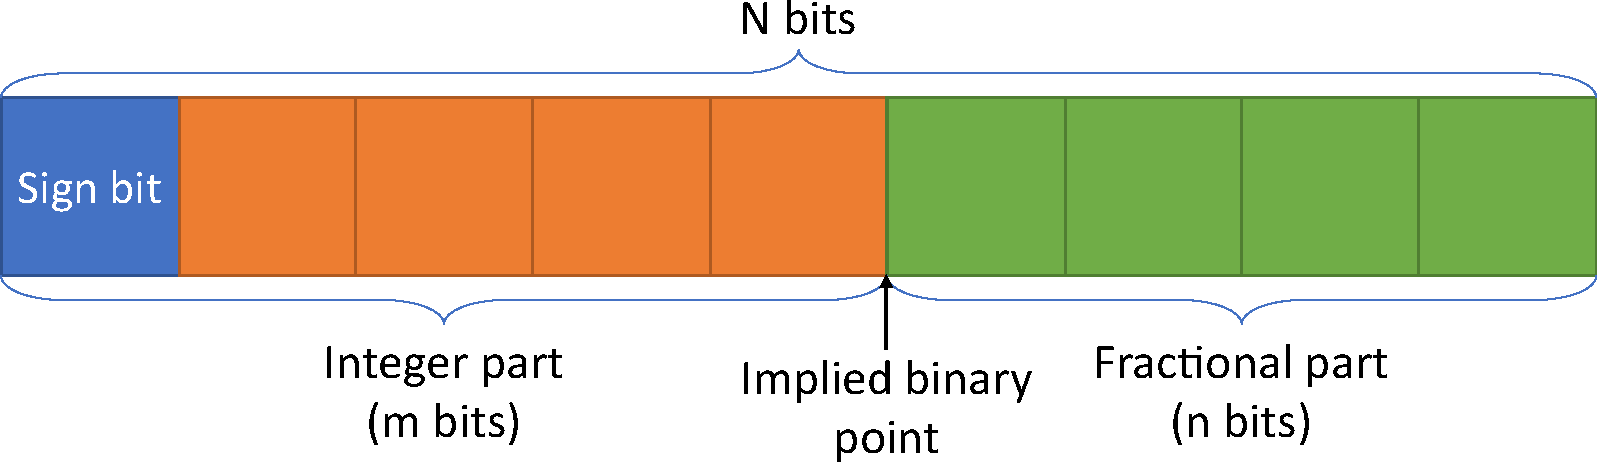
\includegraphics[width=\textwidth]{Qformat.pdf}
    \caption{Illustration of the Q-format}
    \label{fig:Qformat}
\end{figure}

As pointed out by \textcite{han_deep_2016}, quantization and pruning techniques are orthogonal and can be combined to compress further the network. Unfortunately, not all existing networks are friendly for quantization, like MobileNet. MobiletNet with quantized pixels and weights has a large drop of accuracy compared with its Non-quantized version (70.50\% using floating-point model vs 1.80\% using an 8-bit pipeline) \cite{sheng_quantization-friendly_2018}. However, the work of \textcite{sheng_quantization-friendly_2018} showed that the source of the accuracy drop was the design of the separable convolution core layer. They proposed therefore a new quantization-friendly separable convolution core layer. Works on MobileNetV2 should then be done to verify the fixed-point inference accuracy. Still, an 8-bit pipeline might not be optimal for MobilNetV2 as increasing the bitwidth to 16-bit could boost accuracy \cite{cheng_recent_2018}. This bitwidth is also widely used \cite{huimin_li_high_2016, bai_cnn_2018}. 

\textbf{Therefore, 16-bit fixed-point Q-format is adopted for input data, weights, and intermediate data in the frame of this thesis}. \textbf{Moreover, as said previously in Section \ref{subs:acti}, we can limit the integer part to 3 bits (one bit is added to express the sign of the weights), and we can use $Q_{4.12}$.}

